\chapter{仙人掌图表示法标准化算法}

仙人掌图表示法保留了原图所有的最小割信息,
因此如果能差分隐私地输出图的仙人掌图表示法,
那么也就完成了差分隐私下近似最小割的求解。
然而,Dinitz的论文\cite{dinitz1976structure}中提供的仙人掌图表示法定义
存在一定局限性,为隐私化带来了障碍。
本章将从仙人掌图表示法的定义出发,
给出一个仙人掌图表示法的标准化算法,
为差分隐私下的最小割问题的分析提供理论基础。

\section{Dinitz仙人掌图表示法简述}

根据定义\ref{cactus},给定任意带权图$G$,存在仙人掌图$\Gamma$和映射$\varphi$作为其仙人掌图表示法。
首先,我们给出最小割在仙人掌图表示法中的表示形式。

\begin{definition}[割的平行与相交]
  设 $R = (X, Y)$和 $R' = (X', Y')$是图中的不同割,它们的相对位置存在两种可能情况:
  \begin{itemize}
    \item 集合 $X \cap X'$、 $X \cap Y'$、 $Y \cap X'$、 $Y \cap Y'$均非空;
    \item 这些集合中存在空集。
  \end{itemize}
  在第一种情况下,割 $R$和 $R'$被称为相交的一对割,在第二种情况下,它们被称为平行的一对割。
\end{definition}
\begin{figure}[htb]
  \centering
  \subfloat[相交的一对割]{
    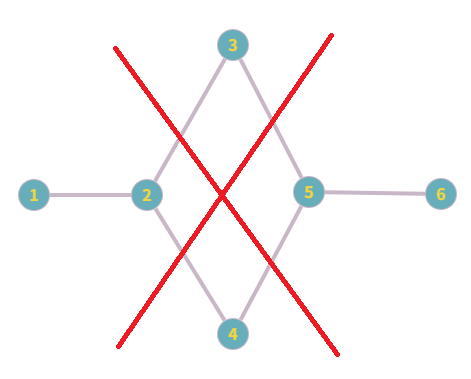
\includegraphics[height=5cm]{figures/graph006.png}}\hspace{4em}
  \subfloat[平行的一对割]{
    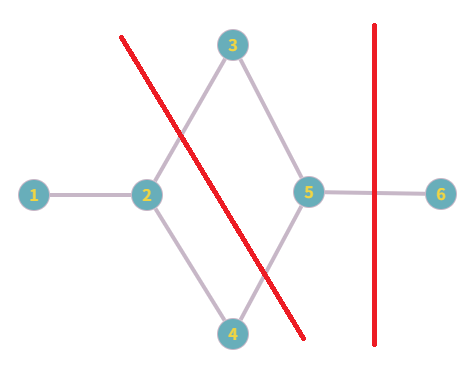
\includegraphics[height=5cm]{figures/graph007.png}}
  \caption{割的平行与相交例}
  \label{crosscut}
\end{figure}
图\ref{crosscut}给出了割相交和平行的两个例子,其中的红色直线代表一个割。

\begin{definition}[最小割图]
  给定图$G$和其最小割集$R*(G)$,最小割图按如下方式生成:
  \begin{itemize}
    \item 对于每个最小割$r*(G)\in R*(G)$,在最小割图中新建一个与之相对应的点。
    \item 若两个最小割$r_1*(G),r_2*(G)$相交,则在最小割图中对应的点之间连一条边。
  \end{itemize}
\end{definition}

\begin{lemma}[割的次模性]\cite{cunningham1985minimum}
  给定图$G=(V,E)$和图的两个割$\Delta(X),\Delta(Y)$,有
  \begin{equation*}
    w(X)+w(Y)\geq w(X\cup Y)+w(X\cap Y)
  \end{equation*}
\end{lemma}

\begin{lemma}[次模性推论]
  给定图$G$和图中两个相交的割$\Delta(X),\Delta(Y)$,则有如下结论:
  \begin{itemize}
    \item $w(X\cap Y)=\Phi_G$
    \item $w(X\cap Y,X\cap (V\backslash Y))=\frac {\Phi_G}2$
    \item $w(X\cap Y,(V\backslash X)\cap (V\backslash Y))=0$
  \end{itemize}
\end{lemma}
\begin{proof}
  根据割的次模性,我们可以得到
  \begin{equation*}
    2\Phi_G\leq w(X\cup Y)+w(X\cap Y)\leq w(X)+w(Y) = 2\Phi_G
  \end{equation*}
  因此,$w(X\cup Y)=w(X\cap Y)=\Phi_G$,第一条结论得证。

  根据第一条结论的对称性,
  $w(X\cap Y)=w(X\cap (V\backslash Y))=\Phi_G$;由于$\Delta(Y)$是最小割,所以$w(Y)=\Phi_G$。
  根据$w$的定义,有
  \begin{equation*}
    w(X\cap Y)+w(X\cap (V\backslash Y))=w(Y)+2w(X\cap Y,X\cap (V\backslash Y))
  \end{equation*}
  因此,$w(X\cap Y,X\cap (V\backslash Y))=\frac {\Phi_G}2$,第二条结论得证。

  根据第二条结论的对称性$ w(X\cap Y,X\cap (V\backslash Y))+w(X\cap Y,(V\backslash X)\cap Y)=\frac{\Phi_G}2$。
  根据$w$的定义,有
  \begin{equation*}
    w(X\cap Y,X\cap (V\backslash Y))+w(X\cap Y,(V\backslash X)\cap Y)+w(X\cap Y,(V\backslash X)\cap (V\backslash Y))=w(X\cap Y)=\Phi_G
  \end{equation*}
  因此,$w(X\cap Y,(V\backslash X)\cap (V\backslash Y))=0$,第三条结论得证。
\end{proof}

\begin{definition}[$p$割与$t$割]
  如果图$G$的一个最小割$R$与其他任何最小割都平行,我们就称它为$p$割;否则,称它为$t$割。
\end{definition}
\begin{figure}[htb]
  \centering
    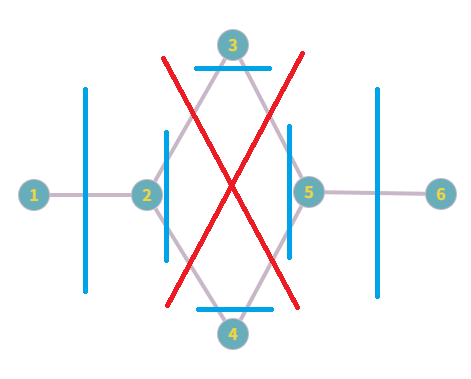
\includegraphics[height=5cm]{figures/graph008.png}
  \caption{$p$割和$t$割例}
  \label{ptcut}
\end{figure}
图\ref{ptcut}给出了图中的所有$p$割(用蓝色直线表示)和$t$割(用红色直线表示)。

\begin{definition}[处于两个$p$割之间的点和割]
  给定两个$p$割$R=(X,Y)$和$R'=(X',Y')$,
  不妨假设$X\cap Y'=\emptyset$。
  我们称点$v$处于$R$和$R'$之间当且仅当$v\in X'\cap Y$。
  我们称割$R''=(X'',Y'')$处于$R$和$R'$之间当且仅当 $X\subset X''$且$Y'\subset Y''$。
\end{definition}


\begin{figure}[htb]
  \centering
    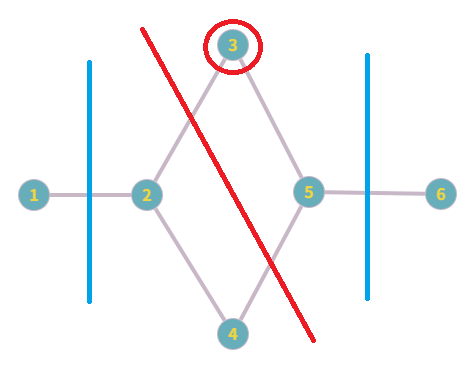
\includegraphics[height=5cm]{figures/graph009.png}
  \caption{处于两个$p$割之间的点和割例}
  \label{between}
\end{figure}
图\ref{between}中红色点以及红色代表的割处于两个蓝色直线表示的$p$割之间。

\begin{definition}[相邻的$p$割]
  给定两个$p$割$R$和$R'$,我们称它们相邻当且仅当不存在处于它们之间的$p$割。
\end{definition}
对于一个$p$割$R=(X,V\backslash X)$,我们记$S(X)$为所有与$R$相邻且分隔开$X$中顶点的割的集合。
\begin{definition}[$p$束]
  给定一个$p$割集合$S$,我们称其为$p$束当且仅当
  存在一个$p$割$R=(X,V\backslash X)$满足$S=S(X)\cup \{R\}$。
  特别的,当$S$中仅包含一个$p$割$R=(X,V\backslash X)$时,该$p$束为叶$p$束,我们用$X_S$表示,该$p$束由$R$的$X_S$一侧得到。
\end{definition}
图的所有$p$束可以通过枚举所有$p$割以及其两侧得到,也就是说,图的$p$束集合是有限且唯一确定的。

\begin{definition}[$p$束内部的顶点和$t$割]
  顶点$v$属于$p$束$S$当且仅当其在$S$中任意两个$p$割之间,$S$此类顶点的集合记作$V(S)$。
  $t$割属于$p$束$S$当且仅当其在$S$中任意两个$p$割之间。
  特别的,对于叶$p$束$S$,顶点$v$属于$S$当且仅当$v\in X_S$。
\end{definition}
这里需要特别说明的是,$t$割不会属于任何叶$p$束,这是由割的次模性推论得到的。
\begin{definition}[相邻的$p$束]
  两个$p$束$S,S'$相邻当且仅当$S\cap S'$非空。
\end{definition}
当$S,S'$相邻时,$S\cap S'$中的元素$R$是唯一的,且$S,S'$分别位于$R$的两侧。
\begin{theorem}[树表示法]\cite{dinitz1976structure}
  \label{treerepresentation}
  给定带权图$G$,存在一个棵树$\Lambda$和映射$\phi:V_G\rightarrow V_\Lambda$,满足:
    \begin{itemize}
        \item 对于点$v_1,v_2\in V_G$,$\phi(v_1)=\phi(v_2)$当且仅当图$G$不存在$p$割$R=(V_1,V_2)$使得$v_1\in V_1,v_2\in V_2$;
        \item 图$G$的最小割$R=(V_1,V_2)$与图$\Lambda$的最小割$(\phi(V_1),V_\Lambda\backslash\phi(V_1))$一一对应。
    \end{itemize}
\end{theorem}

\begin{theorem}[树表示法的性质]\cite{dinitz1976structure}
  \label{treerepresentation2}
  图$G$的树表示法$\Lambda$有以下两个性质:
  \begin{itemize}
    \item $\Lambda$上每一条边的边权都等于最小割的割值。
    \item $\Lambda$中的点与$p$束一一对应,边与$p$束的相邻关系一一对应。
  \end{itemize}
\end{theorem}

\begin{lemma}[树表示法的唯一性]
  \label{treeunique}
  给定带权图$G$,其树表示法$(\Lambda,\phi)$唯一。
\end{lemma}
\begin{proof}
  使用反证法,不妨假设图$G$有两个不相同的树表示法$(\Lambda,\phi)$和$(\Lambda',\phi')$。
  首先,根据定理\ref{treerepresentation}的第一条性质,若存在$v_1,v_2\in V_G$满足$\phi(v_1)=\phi(v_2)$但$\phi(v_1)\neq\phi(v_2)$,
  则将两点分隔开的$p$割的存在性出现矛盾。因此$\phi=\phi'$。

  图$G$的$p$束集合有限且唯一确定,而根据定理\ref{treerepresentation2}可得
  $\Lambda$中的点与$G$的$p$束一一对应,且边与$p$束的相邻关系一一对应,因此
  $\Lambda$与$\Lambda'$相同。综上,$(\Lambda,\phi)$和$(\Lambda',\phi')$是同一个树表示法。
\end{proof}


\begin{definition}[原子]
  给定图$G=(V,E)$和$G$中割的集合$\mathcal{C}$。$\mathcal{C}$的原子是一个$V$的划分$P$的所有划分块,其中$P$满足
  \begin{itemize}
    \item 对于任意割$(X,V\backslash X)\in \mathcal{C}$以及任意原子$A\in P$,满足$A\subseteq X$或$A\subseteq V\backslash X$。
    \item $P$是满足条件的最粗划分,也就是说对于任何满足条件的划分$P'$,都有$P'\preceq P$。
  \end{itemize}
\end{definition}

通俗来讲,一组割会将图的点集划分成若干个划分块,每个划分块就是一个原子。

\begin{theorem}[最小割和$p$割对应的原子集等价]\cite{dinitz1976structure}
  给定图$G$,由所有最小割构成的割集得到的原子集和由所有$p$割构成的割集得到的原子集等价。
\end{theorem}

\begin{definition}[$p$束结构图$G_S$]
定义$G_S$为图$G$中$p$束$S$的结构图,其生成方式如下:
\begin{itemize}
  \item 将$G_S$初始化为$G$。
  \item 枚举$S$中的$p$割$R$,并对被该割与$S$分隔开的点集执行点收缩(同时记收缩得到的点为$x_R$)。
\end{itemize}
\begin{definition}[$\hat c$环]
  所有边的权重都为 $\hat{c}/2$的环被称为 $\hat{c}$环。 
\end{definition}
\end{definition}
\begin{theorem}[含$t$割的$p$束的结构图为环]\cite{dinitz1976structure}
  \label{ring}
  如果一个 $p$ 束 $S$存在内部的$t$割,
  那么图 $G_S$是以顶点 $x_R$( $R\in S$)构成的 $\hat{\Phi_G}$环 。
\end{theorem}
定理\ref{ring}说明了当$p$束$S$内存在$t$割的情况,其核心结论主要有两点。第一个结论是当$S$内存在$t$割时,
则$V(S)=\emptyset$,这是由$\hat{\Phi_G}$环仅由$x_R$即$S$外部的顶点构成这一结果得到的;
第二个结论是$S$内的$t$割恰好是将环分成两部分的割(需满足每一部分至少有两个点),且这些$t$割在最小割图中恰好构成一个联通块。

通过上述定义与定理可以发现,仙人掌图表示法用非环边表示$p$割,用环边二元组表示$t$割。



\section{仙人掌图表示法的不唯一性}

考虑仙人掌图表示法中映射$\varphi$的逆映射$\varphi^{-1}$,该逆映射是从$V_\Gamma$到$\mathcal{P}(V_G)$的映射,
通俗的说,$\Gamma$中的点对应着$G$中的$0$个、$1$个或多个点。
首先,我们形式化的定义仙人掌图表示法的等价性。

\begin{definition}
  \label{cactusequal}
  给定点集$V$,仙人掌图表示法由仙人掌图$\Gamma$和映射$\varphi:V\rightarrow V_\Gamma$构成,
  其对应的割集为
  \begin{equation*}
    CutSet(\Gamma,\varphi)=\{(X,Y)\in R^*_{\Gamma}|(\bigcup_{x\in X}\varphi^{-1}(x),\bigcup_{y\in Y}\varphi^{-1}(y))\}
  \end{equation*}
  两个仙人掌图表示法$(\Gamma,\varphi),(\Gamma',\varphi')$等价当且仅当$CutSet(\Gamma,\varphi)=CutSet(\Gamma',\varphi')$。
\end{definition}

这个定义从侧面表明,一个仙人掌图表示法对应了原图的一个割集。但是,一个原图的割集可能对应多个仙人掌图表示法。

\begin{lemma}
  \label{cactusnonunique}
  图的仙人掌图表示法不具有唯一性。
\end{lemma}
\begin{proof}
  想要证明这一点,我们只需要给出一个图$G$以及其两个不相同的仙人掌图表示法$(\Gamma,\varphi),(\Gamma',\varphi')$。
  \begin{figure}[htb]
    \centering
    \subfloat[图$G$]{
      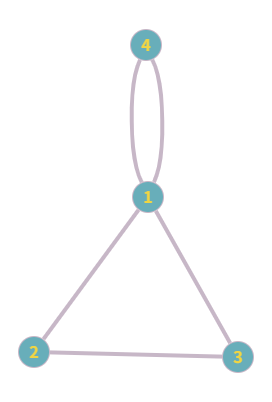
\includegraphics[height=5cm]{figures/graph003.png}}\hspace{4em}
    \subfloat[图$\Gamma$]{
        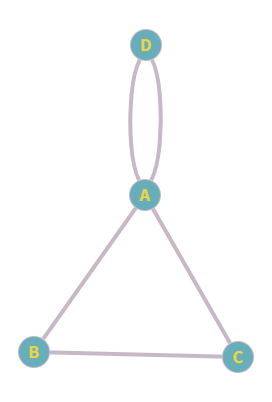
\includegraphics[height=5cm]{figures/graph004.png}}\hspace{4em}
    \subfloat[图$\Gamma'$]{
      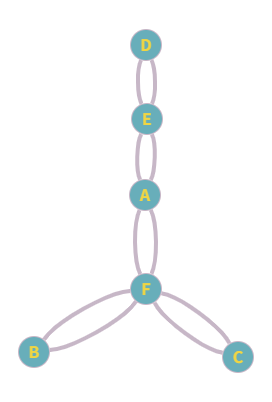
\includegraphics[height=5cm]{figures/graph005.png}}
    \caption{同一个图的两种仙人掌图表示法}
\end{figure}

我们给出了一个$n=4$的例子,$G,\Gamma,\Gamma'$的结构如图所示,且映射满足
\begin{equation*}
  \varphi=\varphi'=\{(1,A),(2,B),(3,C),(4,D)\}
\end{equation*}
在这个例子中,原图的最小割有$(\{1,4\},\{2,3\}),(\{1,2,4\},\{3\}),(\{1,3,4\},\{2\}),(\{1,2,3\},\{4\})$。
仙人掌图表示法$(\Gamma,\varphi)$使用了与图$G$相同的结构,因此其最小割与原图的最小割一一对应。
仙人掌图表示法$(\Gamma',\varphi')$进行了两个改动:
第一个改动是通过加入节点$F$,使$A,B,C$构成的三元环变成三个二元环,
三元环所表示的最小割分别转而由这三个二元环所表示,所以该改动不影响割集
以割$(\{1,3,4\},\{2\})$为例,其由$\Gamma$中的三元环边$(A,B),(B,C)$共同表示,
而到了$\Gamma'$中,其转而由两条$(B,F)$边构成的二元环表示;
第二个改动是在$A$和$D$之间加入$E$,这使得$\Gamma'$中的最小割数量增加,
即$(\{A,B,C,F\},\{D\})$扩展成了$(\{A,B,C,F\},\{D,E\})$和$(\{A,B,C,E,F\},\{D\})$两个最小割,
然而由于$\varphi^{-1}(E)=\emptyset$,因此这两个$\Gamma'$中的割对应$G$的同一个割,改动不影响割集。
综上,$(\Gamma,\varphi),(\Gamma',\varphi')$都是$G$的仙人掌图表示法,图的仙人掌图表示法不具有唯一性。
\end{proof}

虽然图的仙人掌图表示法不具有唯一性,但其仙人掌图表示法相互等价,
这是由表示的最小割集的唯一性得出的。
因此,如果在仙人掌图表示法的生成算法中加入仙人掌图表示法的标准化算法$ALG_{std}$,
将输出的仙人掌图表示法转化为其等价类的标准元,
那么就可以确保算法输出的唯一性。

特别的,仙人掌图表示法的标准化在差分隐私下尤为重要。
对于最小割集相同的边相邻图,算法得到的仙人掌图表示法可能因边集的差异而不同,
而在标准化处理后,输出将正确地被判定为相同。

\section{标准化仙人掌图表示法}

本节中,仙人掌图表示法的标准化共分为两部分。
第一步是通过给出构造方法定义仙人掌图表示法的标准元。
第二步是给出将现有仙人掌图表示法转化为其标准元的高效算法。

根据引理\ref{treeunique},树表示法$\Lambda$可以表示所有$p$割且方法唯一。
根据定理\ref{ring},$p$束的结构图可以表示该$p$束的所有$t$割且方法唯一。
因此,如果将树表示法和每个$p$束的结构图进行合成得到的图也是唯一的,且恰好能表示所有的最小割,
我们将这个图设置为该仙人掌图表示法的标准元。
算法\ref{alg:gen}给出了$ALG_{gen}$的具体实现。我们称$ALG_gen(G)$为图$G$的标准仙人掌图表示法。

\begin{algorithm}
  \caption{图$G$的仙人掌图表示法构造算法$ALG_{gen}$}
  \label{alg:gen}
  \begin{algorithmic}[1] % [1] 表示从第1行开始编号
  \Statex 输入:图$G$
  \Statex 输出:仙人掌图表示法$(\Gamma,\varphi)$
  \State 计算图$G$的$p$割,$t$割。
  \State 计算图$G$中的所有$p$束。
  \State 为每个$p$束$S$新建一个$\Gamma$中的点$v_S$,并更新$S$内的点到$v_S$的映射$\varphi$。
  \State 若两个$p$束$S,S'$相邻,则为其在$\Gamma$中的点$v_S,v_{S'}$连一条边,得到图$G$的树表示法。
  \State 若$p$束$S$中有$t$割,则将$v_S$替换为$G_S$,原本连向$v_S$的代表$p$割$R$的边重新连向$G_S$中的点$x_R$。
  \State \Return $(\Gamma,\varphi)$
  \end{algorithmic}
\end{algorithm}

\begin{theorem}
  给定图$G,G'$,其仙人掌图表示法分别为$(\Gamma,\varphi)$和$(\Gamma',\varphi')$。
  若$(\Gamma,\varphi)$和$(\Gamma',\varphi')$等价,则$ALG_{gen}(G)=ALG_{gen}(G')$
\end{theorem}

\begin{proof}
  $(\Gamma,\varphi)$和$(\Gamma',\varphi')$等价,则根据定义\ref{cactusequal},有 $CutSet(\Gamma,\varphi)=CutSet(\Gamma',\varphi')$。
  由仙人掌图表示法的定义,
  $CutSet(\Gamma,\varphi)$和$CutSet(\Gamma',\varphi')$分别对应$\Gamma$的最小割集和$\Gamma'$的最小割集。
  $ALG_{gen}(G)$的仅与$G$的最小割集有关,因此$ALG_{gen}(G)=ALG_{gen}(G')$。

\end{proof}

算法$ALG_{gen}(G)$给出了仙人掌图表示法的标准元,但难以直接用于仙人掌图表示法构造算法中。
因为算法没有提供一个高效的计算方法,而朴素的$p$割,$t$割,$p$束计算需要较高复杂度,继而成为算法的效率瓶颈。

我们发现,如果我们首先利用现有工作生成一个仙人掌图表示法,然后使用仙人掌图表示法标准化算法$ALG_{std}$,
将仙人掌图表示法转化为其等价类内的标准元,那么就能同时实现高效和标准化。
与此同时,$ALG_{std}$可以通过输入仙人掌图表示法本身的性质,来得到一个较好的复杂度。


\begin{algorithm}
  \caption{仙人掌图表示法标准化算法$ALG_{std}$}
  \label{algstd}
  \begin{algorithmic}[1] % [1] 表示从第1行开始编号
  \Statex 输入:仙人掌图表示法$(\Gamma,\varphi)$
  \Statex 输出:仙人掌图表示法$(\Gamma',\varphi')$
  \State 设仙人掌图表示法$(\Gamma,\varphi)$的最小割的割值为$c$
  \State 对于所有二元环,将环上的两条边合并为一条边。\Comment{二元环表示$p$割}
  \For {$\Gamma$中的简单环$C$}
      \For {$C$中的节点$k$}
          \State 在$\Gamma$中新建顶点$k',k''$来替换$k$
          \State 令$\varphi^{-1}(k'')=\varphi^{-1}(k),\varphi^{-1}(k')=\emptyset$
          \State 在$k',k''$之间连一条边权为$c$的边
          \For {与$k$相连的边$e$}
            \If{$e$是环$C$上的边}
                \State 将$e$的$k$一端替换成$k'$
            \ElsIf{$e$是环$C$上的边}
                \State 将$e$的$k$一端替换成$k''$
            \EndIf
          \EndFor
      \EndFor
  \EndFor
  \State 对$\Gamma$中的所有三元环执行点收缩。\Comment{三元环只表示$p$割}
  \For {$\Gamma$中度数为$2$的点$v$}
      \State 找到与$v$相连的边$(v,u_1),(v,u_2)$
      \If{若$v$不处于任何一个简单环上且$\varphi^{-1}(v)=\emptyset$}
          \State 删除点$v$以及与其相连的边
          \State 加入边$(u_1,u_2)$
      \EndIf
  \EndFor
  \State \Return $(\Gamma',\varphi')$
  \end{algorithmic}
\end{algorithm}

回顾引理\ref{cactusnonunique}中的例子,仙人掌图表示法主要需要解决的是三元环和链两种情况。
算法\ref{algstd}给出了$ALG_{std}$的具体实现。

\begin{theorem}
  给定图$G$和其仙人掌图表示法$(\Gamma,\varphi)$,则$ALG_{std}((\Gamma,\varphi))=ALG_{gen}(G)$
\end{theorem}

\begin{proof}
  首先,我们分析仙人掌图表示中,单个环表示的最小割的数量和类型。根据定理\ref{ring}

  首先,我们需要证明$ALG_{std}((\Gamma,\varphi))$算法得到的环与$ALG_{gen}(G)$的环一一对应。
  在仙人掌图表示中,非环边代表的最小割一定是$p$割,环中代表的最小割可能有$p$割也可能有$t$割。
  根据算法\ref{alg:gen}可知,$ALG_{gen}(G)$的环仅用于表示$t$割。对于一个$ALG_{gen}(G)$里的简单环$C$,
  若其表示的$t$割在最小割图中恰好构成一个连通块,因此这些割在$(\Gamma,\varphi)$中
  一定由一个相同的环$C'$表示。对于一个仙人掌图表示$(\Gamma,\varphi)$中的环$C'$,环上相邻的两条边可以表示一个$p$割,
  这些$p$割在算法中通过$(k',k'')$这条非环边重新表示了;
  若环$C'$不表示任何$t$割,那么其一定是一个二元环或三元环,在算法中被消除。
  综上,$ALG_{std}((\Gamma,\varphi))$算法得到的环与$ALG_{gen}(G)$的环一一对应。

  接下来,我们证明将所有环缩成点后,
  $ALG_{std}((\Gamma,\varphi))$的树结构和$ALG_{gen}(G)$的树结构相同。
  $(\Gamma,\varphi)$的$p$割由非环边和环共同表示,而在处理环的过程中,
  所有环表示的$p$割转而以$(k',k'')$的形式表示。因此,处理完环之后,$(\Gamma,\varphi)$的树结构和$ALG_{gen}(G)$
  都能表示所有$p$割。$(\Gamma,\varphi)$的树结构表示了所有$p$割,但不一定是树表示法,
  因为树表示法的边与$p$割一一对应,但是树结构可以存在多条边对应同一个$p$割。
  由于代表同一个$p$割的两条边之间的树上路径的点$v$都满足$\varphi^{-1}=\emptyset$,
  因此,$ALG_{std}$通过收缩这样的点,就可将树结构转化为树表示法。
  根据定理\ref{treerepresentation},树表示法具有唯一性。
  综上, $ALG_{std}((\Gamma,\varphi))$的树结构和$ALG_{gen}(G)$的树结构相同。

  最终,结合以上两个结果,可以得出$ALG_{std}((\Gamma,\varphi))=ALG_{gen}(G)$。
\end{proof}